\documentclass[12pt,letterpaper]{article}

% Essential packages
\usepackage[margin=1in]{geometry}
\usepackage{amsmath,amsthm,amssymb}
\usepackage{graphicx}
\usepackage{booktabs}
\usepackage{xcolor}
\usepackage{tcolorbox}
\usepackage{fancyhdr}
\usepackage{titlesec}
\usepackage{hyperref}
\usepackage{enumitem}
\usepackage{tikz}
\usepackage{lipsum} % For demo text only

% Define colors
\definecolor{chaptercolor}{HTML}{1B5E20}
\definecolor{examplecolor}{HTML}{E3F2FD}
\definecolor{exampleborder}{HTML}{1E88E5}
\definecolor{keyideacolor}{HTML}{FFF3E0}
\definecolor{keyideaborder}{HTML}{FF9800}
\definecolor{remarkcolor}{HTML}{F3E5F5}
\definecolor{remarkborder}{HTML}{9C27B0}

% Style the chapter headings
\titleformat{\section}
{\normalfont\LARGE\bfseries\color{chaptercolor}}
{\thesection}{1em}{}[\titlerule]

% Custom environments
\newcounter{example}[section]
\newenvironment{example}
{\refstepcounter{example}\par\medskip
   \begin{tcolorbox}[colback=examplecolor,
                     colframe=exampleborder,
                     arc=0mm,
                     title=Example~\theexample]
}
{\end{tcolorbox}\par\medskip}

\newcounter{keyidea}[section]
\newenvironment{keyidea}
{\refstepcounter{keyidea}\par\medskip
   \begin{tcolorbox}[colback=keyideacolor,
                     colframe=keyideaborder,
                     arc=0mm,
                     title=Key Idea~\thekeyidea]
}
{\end{tcolorbox}\par\medskip}

\newcounter{remark}[section]
\newenvironment{remark}
{\refstepcounter{remark}\par\medskip
   \begin{tcolorbox}[colback=remarkcolor,
                     colframe=remarkborder,
                     arc=0mm,
                     title=Remark~\theremark]
}
{\end{tcolorbox}\par\medskip}

% Style footnotes with symbols
\renewcommand{\thefootnote}{\fnsymbol{footnote}}

% Header and footer
\pagestyle{fancy}
\fancyhf{}
\fancyhead[L]{\textit{\bookname}}
\fancyhead[R]{\textit{Chapter \thesection}}
\fancyfoot[C]{\thepage}
\renewcommand{\headrulewidth}{0.4pt}
\renewcommand{\footrulewidth}{0.4pt}

% Document title and information
\newcommand{\bookname}{}
\newcommand{\booknotes}[3]{
    \renewcommand{\bookname}{#1}
    \title{\textbf{\Huge{Notes on:}\\\Huge{\textcolor{chaptercolor}{#1}}}}
    \author{#2}
    \date{#3}
}

\begin{document}

\booknotes{Mathematical Analysis}{Your Name}{Spring 2025}
\maketitle
\tableofcontents
\newpage

\section{Introduction to Real Analysis}

This chapter covers the foundations of real analysis, beginning with properties of the real number system.

\begin{keyidea}
    The completeness property of real numbers states that every non-empty set of real numbers that is bounded above has a least upper bound.
\end{keyidea}

\begin{example}
    Consider the set $S = \{x \in \mathbb{R} : x^2 < 2\}$. 
    This set is bounded above, and its least upper bound is $\sqrt{2}$.
    
    We can verify this by noting that:
    \begin{itemize}
        \item If $x^2 < 2$, then $x < \sqrt{2}$, so $\sqrt{2}$ is an upper bound.
        \item For any $\varepsilon > 0$, $(\sqrt{2} - \varepsilon)^2 < 2$, so $\sqrt{2} - \varepsilon \in S$.
    \end{itemize}
    
    Therefore, $\sqrt{2}$ is the least upper bound of $S$.
\end{example}

\begin{remark}
    The completeness property distinguishes the real numbers from the rational numbers. For instance, the set $\{x \in \mathbb{Q} : x^2 < 2\}$ has no least upper bound in $\mathbb{Q}$.
\end{remark}

Here's a visual representation of the concept of least upper bound:

\begin{figure}[h]
    \centering
    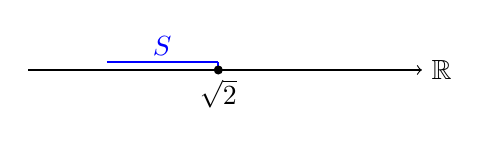
\begin{tikzpicture}
        \draw[->] (-1,0) -- (4,0) node[right] {$\mathbb{R}$};
        \draw[thick, blue] (0,0.1) -- (1.414,0.1);
        \draw[thick, blue] (1.414,0.1) -- (1.414,0);
        \draw[fill] (1.414,0) circle (0.05) node[below] {$\sqrt{2}$};
        \node[blue] at (0.7,0.3) {$S$};
    \end{tikzpicture}
    \caption{The set $S = \{x \in \mathbb{R} : x^2 < 2\}$ with least upper bound $\sqrt{2}$}
    \label{fig:lub}
\end{figure}

A proper understanding of completeness\footnote{This concept was first rigorously formulated by Dedekind in the 19th century.} is essential for developing the theory of limits and continuity.

\newpage
\section{Sequences and Series}

In this chapter, we explore infinite sequences and series, their convergence properties, and tests for convergence.

\begin{keyidea}
    A sequence $\{a_n\}$ converges to a limit $L$ if for every $\varepsilon > 0$, there exists $N \in \mathbb{N}$ such that $|a_n - L| < \varepsilon$ for all $n \geq N$.
\end{keyidea}

\begin{example}
    Let's prove that the sequence $a_n = \frac{1}{n}$ converges to 0.
    
    Given $\varepsilon > 0$, we need to find $N$ such that $|\frac{1}{n} - 0| < \varepsilon$ for all $n \geq N$.
    
    Since $|\frac{1}{n} - 0| = \frac{1}{n}$, we need $\frac{1}{n} < \varepsilon$, which is equivalent to $n > \frac{1}{\varepsilon}$.
    
    Therefore, we can choose $N = \lceil\frac{1}{\varepsilon}\rceil$, and for all $n \geq N$, we have $|a_n - 0| < \varepsilon$.
\end{example}

\begin{remark}
    While many sequences converge, there are important examples of divergent sequences like $a_n = (-1)^n$ and $a_n = n$.
\end{remark}

\end{document}